\begin{pastexam}[label={px:ccu-114-csb-10}]{中正資工所乙組 114 學年度 第 10 題}
（單選）

(5\%) Find the sequence in which Prim's algorithm adds edges to the minimum spanning tree for the graph shown below, starting with vertex $A$. If two unvisited vertices have the same cost during the algorithm, chose the one with the smaller alphabetical order. Use the format (node1, node2) to represent each edge.

\begin{center}
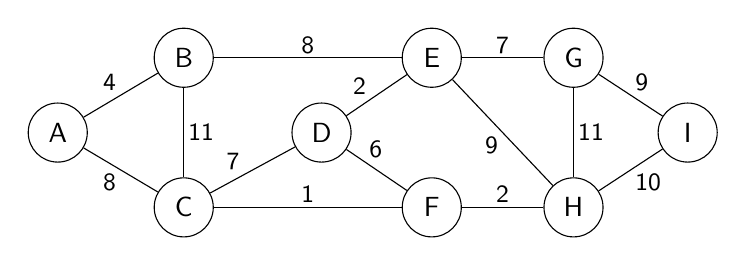
\begin{tikzpicture}[v/.style={circle,draw,minimum size=7.5mm,inner sep=0pt,font=\sffamily},w/.style={font=\sffamily\small,inner sep=1.5pt},x=1cm,y=1cm]
\node[v] (A) at (0,0) {A};
\node[v] (B) at (1.6,0.95) {B};
\node[v] (C) at (1.6,-0.95) {C};
\node[v] (D) at (3.35,0) {D};
\node[v] (E) at (4.75,0.95) {E};
\node[v] (F) at (4.75,-0.95) {F};
\node[v] (G) at (6.55,0.95) {G};
\node[v] (H) at (6.55,-0.95) {H};
\node[v] (I) at (8.0,0) {I};
\draw (A)--node[w,above left]{4}(B);
\draw (A)--node[w,below left]{8}(C);
\draw (B)--node[w,right]{11}(C);
\draw (B)--node[w,above]{8}(E);
\draw (C)--node[w,above left,pos=0.4]{7}(D);
\draw (C)--node[w,above]{1}(F);
\draw (D)--node[w,above left,pos=0.4]{2}(E);
\draw (D)--node[w,above right,pos=0.3]{6}(F);
\draw (E)--node[w,above]{7}(G);
\draw (E)--node[w,below left,pos=0.5]{9}(H);
\draw (F)--node[w,above]{2}(H);
\draw (G)--node[w,right]{11}(H);
\draw (G)--node[w,above right]{9}(I);
\draw (H)--node[w,below right]{10}(I);
\end{tikzpicture}
\end{center}

\begin{enumerate}[label=\Alph*.]
\item (C, F), (D, E), (F, H), (E, H), (A, B), (E, G), (A, C), (G, I)
\item (A, B), (B, E), (E, D), (D, F), (C, F), (F, H), (H, I), (G, I)
\item (A, B), (A, C), (C, D), (C, F), (D, E), (F, H), (E, G), (G, I)
\item (A, B), (B, E), (D, E), (E, H), (F, H), (C, F), (E, G), (G, I)
\item None of the above
\end{enumerate}
\end{pastexam}

\begin{pastsoln}
答案是 E（None of the above）。 正確的加邊順序是
\[
(A, B),\ (A, C),\ (C, F),\ (F, H),\ (D, F),\ (D, E),\ (E, G),\ (G, I),
\]
總權重 $4 + 8 + 1 + 2 + 6 + 2 + 7 + 9 = 39$。

照資結書第~24.3~節的 Prim 演算法：維護每個樹外頂點連到樹的最小邊權 $\mathit{key}$，每次把 $\mathit{key}$ 最小的頂點（平手取字母小的）
連同那條邊加進樹，再用它的鄰邊更新 $\mathit{key}$。 圖的邊：A--B $4$、A--C $8$、B--C $11$、B--E $8$、C--D $7$、C--F $1$、D--E $2$、
D--F $6$、E--G $7$、E--H $9$、F--H $2$、G--H $11$、G--I $9$、H--I $10$。
\begin{center}
\small
\begin{tabular}{cll}
\toprule
步驟 & 加入的邊 & 加入後樹外頂點的 $\mathit{key}$（括號是另一端） \\
\midrule
1 & (A, B) $4$ & C $8$(A)、E $8$(B) \\
2 & (A, C) $8$ & C、E 平手取 C。 D $7$(C)、E $8$(B)、F $1$(C) \\
3 & (C, F) $1$ & D $6$(F)、E $8$(B)、H $2$(F) \\
4 & (F, H) $2$ & D $6$(F)、E $8$(B)、G $11$(H)、I $10$(H) \\
5 & (D, F) $6$ & E $2$(D)、G $11$(H)、I $10$(H) \\
6 & (D, E) $2$ & G $7$(E)、I $10$(H) \\
7 & (E, G) $7$ & I $9$(G) \\
8 & (G, I) $9$ & （全部在樹裡） \\
\bottomrule
\end{tabular}
\end{center}
第 2 步 C、E 的 $\mathit{key}$ 都是 $8$，依規定取 C。 第 3 步之後 D 的 $\mathit{key}$ 從 $7$（C--D）降到 $6$（F--D），所以加的是 (D, F)，
不是 (C, D)。

逐項檢查：
\begin{itemize}
\item A：第一條是 (C, F)，但 Prim 從 A 開始，第一條邊一定接在 A 上；這是 Kruskal 那種依權重由小到大挑邊的順序。 錯。
\item B：(A, B) 之後加 (B, E)，但那時 C 和 E 平手（都是 $8$），要先取 C；後面的 (H, I) $10$ 也不在最小生成樹裡（(G, I) $9$ 較小）。 錯。
\item C：第三條是 (C, D) $7$，但那時 (C, F) 只要 $1$，應該先加；而且這組邊用 C--D $7$ 而不是 D--F $6$，總權重 $40$，不是最小生成樹。 錯。
\item D：同 B，第二條不該是 (B, E)。 錯。
\item E：正確的順序不在選項中。 對。
\end{itemize}
\end{pastsoln}
